\chapter{Markt \& Wettbewerb}
\label{sec:Marketing}

\section{Gesamtmarkt}
Allein im Jahr 2017 wurde ein Absatz von ca. $294.000$ neuen, industriell genutzten, Robotern erzielt. Bis 2020 wird mit rund $1,7$ Millionen zusätzlichen Robotern gerechnet, was in etwa einer Verdoppelung des derzeitigen Bestandes auf insgesamt $3$ Mio entspricht.

\section{Marktsegmentierung}
\subsection{Hersteller}
Die 5 größten Hersteller in der Roboterbranche sind:
\begin{itemize}
\item FANUC
\item YASKAWA
\item ABB
\item KUKA
\item KAWASAKI
\end{itemize}

\subsection{Märkte}
\subsubsection{Anzahl an Robotern in Absoluten Zahlen}
\begin{itemize}
\item China
\item Korea
\item Japan
\item US
\item Deutschland
\end{itemize}
Diese 5 Länder machen gemeinsam in etwa $75$\% des Gesamtmarktes für industrielle Roboter aus.\\
Weitere relevante Absatzländer sind in der Abbildung \ref{fig:TotalAmountOfRobots} zu sehen:
\begin{figure}[h]
	\centering
	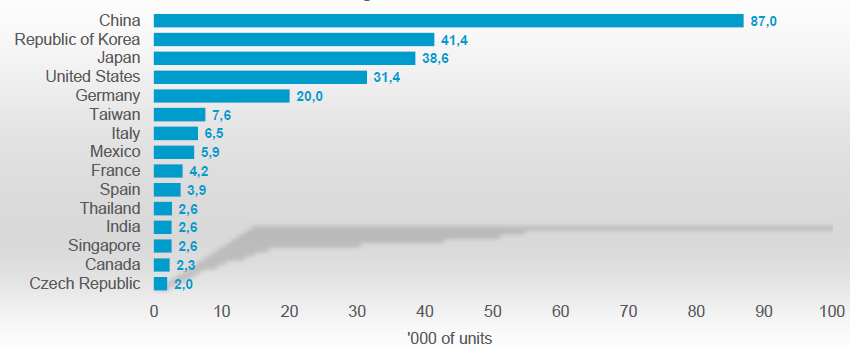
\includegraphics[width=15cm]{TotalAmountOfRobots.png}
	\caption{Geschätzte Anzahl an Robotern der 15 größten Märkte in 2016}
	\label{fig:TotalAmountOfRobots}
\end{figure}
\subsubsection{Roboter in der Automobilindustrie pro 10.000 Arbeitern}
Die Automobilindustrie ist besonders für die Offline-Variante unseres Produkte interessant. Hierbei liegt eine andere Marktkonstellation wie für die restliche Verteilung der in der Industrie eingesetzten Roboter vor. Die genaue Verteilung ist der Grafik \ref{fig:RobotsPer10kWorker} zu entnehmen:
\begin{figure}[h]
	\centering
	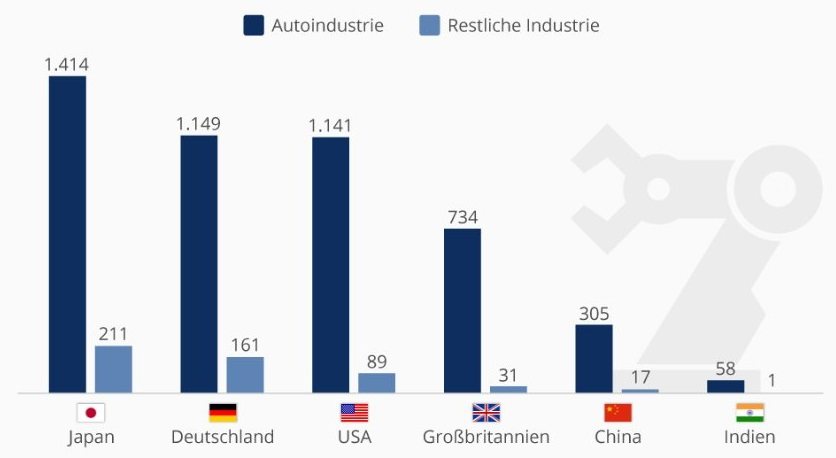
\includegraphics[width=15cm]{RobotsPer10kWorker.jpg}
	\caption{Zahl der Roboter pro 10.000 Angestellten (2014)}
	\label{fig:RobotsPer10kWorker}
\end{figure}

\section{Zielgruppenbeschreibung}
Unsere Hauptzielgruppe sind Firmen, die durch Optimierung der Roboterbahnen Energie sparen wollen. Diese Investition amortisiert sich nicht nur nach kurzer Zeit, sondern reduziert auch den Enegrieverbrauch und damit den ökologischen Fußabrdruck. Dadurch lässt sich das Image insbesondere in Bezug auf Umweltbewusstsein verbessern. Ausserdem ergibt sich ein positiver Effekt bezüglich der Richtlinie 2012/27/EU welche Energieaudits und eine besserung der Energieeffizienz bis 2020 vorschreibt.\\
Durch Entwicklung von Plugins/Libraries für gängige Softwaresuiten der großen Roboterhersteller lässt sich nahezu der gesamte Markt abdecken. Durch entwickeln einer Online-Optimierung für flexible Fertigungszellen und Einsatzgebiete von variierenden Stückzahlen sowie einer Offline-Optimierung für fixe Anwendungen wie Fertigungsstraßen lassen sich unterschiedliche Zielgruppen ansprechen. 

\section{Wettbewerb}
Ein enormer Trend geht derzeit in Richtung Energieeinsparung und energieeffizientere Steuerungen (zb. KUKA Quantec/KR C4, auch FANUC, YASKAWA und KAWASAKI geben an, energiesparendere und effizientere Steuerungen denn je zuvor anzubieten).\\
Andere Ansätze für Verbesserungen wurden bisher nur in einzelnen Tests oder für Forschungszwecke implementiert.\\
Der daher größte derzeit relevante Wettbewerber sind die Roboterhersteller selbst. Diese bauen aufgrund eben dieses Trends Steuerung, die mit intelligenter Optimierung arbeiten, Stromregeneration oder die Dynamik des Roboters besser nutzen. Diese erreichen jedoch nicht das selbe Ausmaß an Verbesserung wie die Lösung von RTI. Eine weitere Verbesserung von durchschnittlich $30$\% sollte möglich sein, diese zusätzliche Einsparung amortisiert sich nach kurzer Zeit.

\section{Eintrittsbarrieren}
Diese sind minimal, aufgrund der in Relation zum Roboter geringen Mehrkosten, welche sich nach 5 Jahren (bei höherer Auslastung bereits früher) amortisieren.

\chapter{Marketing}

\section{Kundenansprache}
Die Hauptargumente, die für unser Produkt sprechen, sind die kurze Amortisationsdauer, die Reduktion der laufenden Energiekosten und die Verbesserung der Energieeffizienz in Hinblick auf die Richtlinie 2012/27/EU, welche bei Energieaudits angeführt werden kann.

\section{Werbemittel, Vertriebs- und Kommunikationskanäle}
Die Hauptkanäle für Vertrieb und Kommunikation sind
\begin{itemize}
\item Messepräsenz
\item Artikel in Fachzeitschriften
\item Direkt als Partner der Roboterhersteller als Zubehör
\item eigene Hompage
\item persönliche Gespräche
\end{itemize}
Besonders für die Offline-Variante bietet sich zusätzlich persönliche Kundenakquise bei einzelnen Großabnehmern an, die viele Roboter in fixen Fertigungsstraßen einsetzen, vor allem in der Automobilbranche ist dieser Aspekt relevant.\\
Die Botschaft bzw. das Ziel der Kommunikation ist die Vermittlung der Idee der Kostenreduktion durch Energieeinsparung und die Imageverbesserung durch umweltfreundlichere Produktion.

\section{Markteintrittsstrategie}
Der wichtigste Punkt der Markteintrittsstrategie ist die Roboterhersteller als Partner zu gewinnen. Diese können auf unser Produkt als Zubehör verweisen, da sich die Anschaffung eines Roboters dieses Herstellers dann schneller amortisiert und somit auch für diese ein gutes Verkaufsargument liefert.